Given the IRT CoDEx-M or FB15k-237 split combined with one of the IRT text sets for that graph, one could already train and evaluate the Power model. However, although Power is capable of open-world prediction due to its Texter component, it only develops its full potential when it can leverage the rules mined from the training facts, which requires some knowledge about the query entity. Therefore an IRT split is transformed to a \emph{Power split} by dividing the IRT split's open-world facts into so-called \emph{known facts}, that are allowed to be used for rule application during inference, and \emph{unknown facts} that stay unknown. This resembles the use case in which the knowledge about a new, partly known entity should be completed. Meanwhile, the close-world entities' training and validation facts are merged as there is no need for the latter. Figure~\ref{fig:5_experiments/2_power_datasets/splits} illustrates how the complete repartitioning.

\begin{figure}[t]
    \centering
    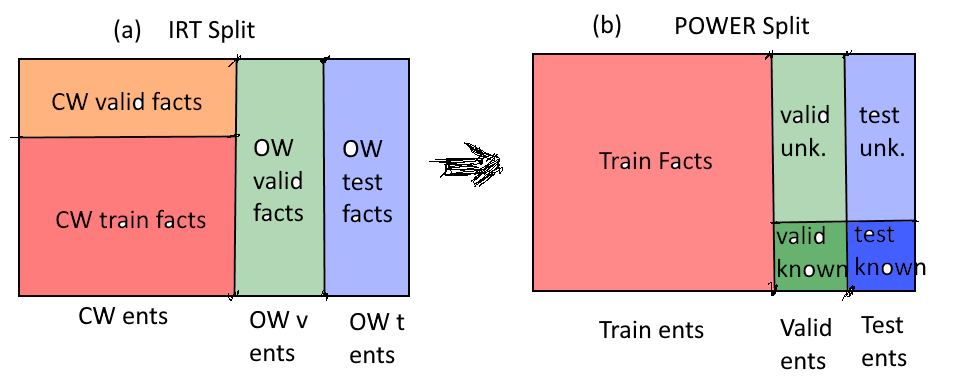
\includegraphics[width=\textwidth]{5_experiments/2_power_datasets/splits}
    \caption{Transforming IRT split into POWER split by merging train facts and splitting valid/test facts}
    \label{fig:5_experiments/2_power_datasets/splits}
\end{figure}

The percentage of known and unknown facts can be varied when creating the Power split to study the Ruler's effectiveness on more or less known entities. Table~\ref{tab:5_experiments/2_power_datasets/power_splits} lists the splits used for the evaluation. In practice, few-shot splits are of particular interest. Since there are only about 20 facts per entity on average, knowing of 5\% or 15\% of these can be considered few-shot scenarios. The splits with 0\% known facts correspond to the zero-shot open-world scenario studied in the IRT paper.

\begin{table}[h]
    \centering
    \begin{tabular}{| l | r | r | r | r | r |}
    \hline
    
    \multicolumn{1}{|c|}{\textbf{Power Split}} &
    \multicolumn{1}{|c|}{\textbf{\thead{Train Facts}}} &
    \multicolumn{1}{|c|}{\textbf{\thead{Known \\ Valid Facts}}} &
    \multicolumn{1}{|c|}{\textbf{\thead{Known \\ Valid Facts \\ per Entity}}} &
    \multicolumn{1}{|c|}{\textbf{\thead{Known \\ Test Facts}}} &
    \multicolumn{1}{|c|}{\textbf{\thead{Known \\ Test Facts \\ per Entity}}} \\

    \hline\hline

    CDE-0   & \multirow{6}{*}{\num{137738}} & \num{0}     & \num{0.00} & \num{0}     & \num{0.00} \\
    CDE-5   &                               & \num{2062}  & \num{0.71} & \num{1378}  & \num{0.73} \\
    CDE-15  &                               & \num{6186}  & \num{2.12} & \num{4136}  & \num{2.18} \\
    CDE-30  &                               & \num{12372} & \num{4.24} & \num{8273}  & \num{4.36} \\
    CDE-50  &                               & \num{20620} & \num{7.07} & \num{13788} & \num{7.27} \\
    CDE-100 &                               & \num{?}     & \num{7.07} & \num{13788} & \num{7.27} \\

    \hline

    FB-0   & \multirow{6}{*}{\num{238191}} & \num{0}     & \num{0.00}  & \num{0}     & \num{0.0} \\
    FB-5   &                               & \num{2325}  & \num{1.50}  & \num{1271}  & \num{1.56} \\
    FB-15  &                               & \num{6975}  & \num{4.51}  & \num{3813}  & \num{4.67} \\
    FB-30  &                               & \num{13950} & \num{9.03}  & \num{7626}  & \num{9.35} \\
    FB-50  &                               & \num{23251} & \num{15.05} & \num{12711} & \num{15.58} \\
    FB-100 &                               & \num{?}     & \num{15.05} & \num{12711} & \num{15.58} \\
    
    \hline
\end{tabular}

    \caption{Power splits}
    \label{tab:5_experiments/2_power_datasets/power_splits}
\end{table}

Combining a Power split with an IRT text set yields a full Power dataset. Training the Texter makes use of the whole Power dataset except for the test entities' facts and texts. For the Ruler, only the Power split is used.
